\chapter{Containerized WebSocket Infrastructure}
\label{chapter:containerizedWebSocketInfrastructure}

This chapter introduces various considerations when deploying WebSocket applications and talks about containerized deployment.

\section{WebSocket Application Deployment}

When deploying a WebSocket application there are requirements that need to be taken into account. These requirements depend on the nature of the deployed applications and the traffic handled by their runtime environments. In addition, devices like reverse proxy servers, firewalls and load-balancing routers must be taken into account when designing and implementing systems that utilize the WebSocket protocol. A large proportion of the internet infrastructure is predominantly configured for HTTP traffic and not familiar with the WebSocket protocol. This can introduce various challenges when deploying applications that utilize.

\subsection{Unencrypted WebSocket Traffic}

The deciding factor whether a client and a server successfully manage to establish an unencrypted WebSocket connection (\texttt{ws://} on port 80) in production environments is usually interaction with proxy servers located on the communication path. Connections through an explicit proxy servers, that a client is explicitly configured to use, will most likely lead to a successful connection upgrade during the WebSocket handshake as they are configured to allow the \texttt{CONNECT} method. When WebSocket traffic flows through transparent proxies it is likely to be dropped as the proxy will likely remove certain header information, like the connection header, which will lead to a failed WebSocket handshake. Even though a transparent proxy server is not configured to remove the connection header the WebSocket connection is still unlikely to succeed as it behaves differently than HTTP traffic which is what the server has been configured for. This will likely be the case until the infrastructure of the internet will more frequently be configured to handle traffic long lived connections of protocols like WebSocket and HTTP/2. Figure x shows interaction between WebSocket and different types of proxy servers and whether a successful connection establishment is likely.
\\
\begin{figure}[h!]
	\centering
	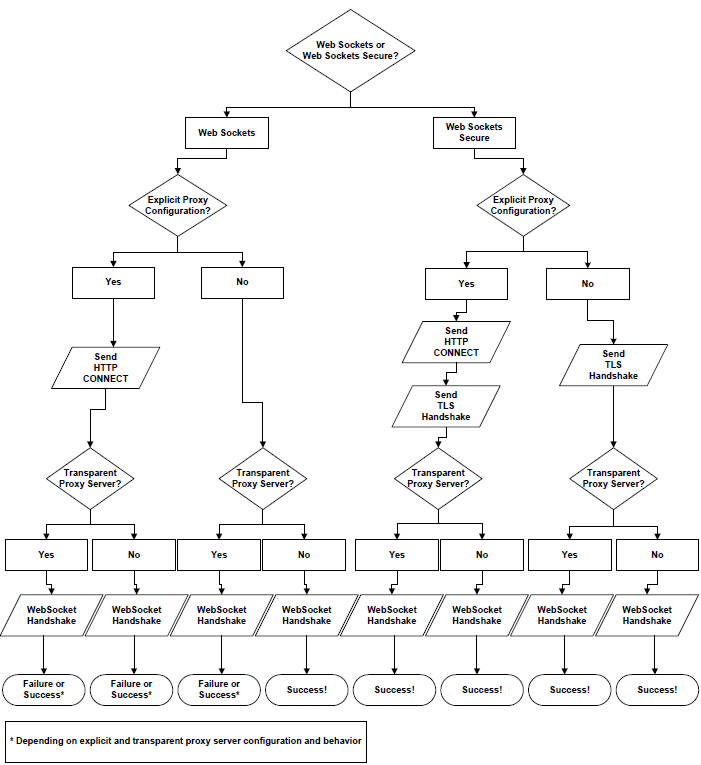
\includegraphics[width=0.9\textwidth]{images/websocketProxyServer}
	\caption{Interaction between WebSocket applications and proxy servers \cite{wang2013definitive}}
	\label{fig:webSocketMessagingSystem}
\end{figure}

\newpage
\subsection{Encrypted WebSocket traffic}

Encrypted WebSocket traffic (\texttt{wss://} on port 443) is more predictable than unencrypted traffic since it is less dependent on the intermediaries on the connection path. In the case of explicit proxies a TLS handshake takes place after a successful WebSocket connection upgrade handshake. Afterwards an encrypted and unhampered WebSocket communication channel is established between a client and a server. When a WebSocket connection is established in the presence of transparent proxies a successful handshake is considerably more likely as the communication is encrypted and proxies are generally configured to accept that kind of traffic. TLS encrypted traffic leads to slightly increased CPU consumption on both sides of the communication but its benefits significantly outweigh that drawback.

\subsection{Fallback Strategies}

In addition to the possible issues proxy servers and other intermediaries can cause for WebSocket traffic some older browsers lack support for the protocol. Currently, all modern browsers \footnote{\url{http://caniuse.com/websocket}} support the protocol but WebSocket applications that are intended for widespread use and corporate environments, where older browsers might be common, should have a decent fallback strategy. Because of the uncertainty in the environment where WebSocket applications can be deployed polyfills, which are libraries that implement a standard API using legacy browser features, can be a good solution. In the case of WebSocket a polyfill library would use HTTP-based communication patterns like polling or long-polling as fallback options. Another option would be to use a plugin, like Adobe Flash, capable of establishing a full-duplex communication channel with TCP sockets. That option use usually the least favorable one as it requires the user to explicitly install the plugin which can lead to a bad user experience.
\\ \\
Engine.io \footnote{\url{https://github.com/Automattic/engine.io}} is a Node.js WebSocket implementation that adds increased reliability when establishing a WebSocket connection between a client and a server. The most important design decision of Engine.io is that communication is initiated with a long-polling connection that is upgraded to better transports that are tested during the first moments of the connection establishment. This approach to WebSocket connection establishment is based on empirical experience working with the protocol in production environments in the vicinity of proxies and other network intermediaries. Experiments even seem to indicate that a WebSocket abstraction like Engine.io can increase data throughput without a significant impact on permornace \cite{ozger2014websocket}. There exists numerous other WebSocket implementations and frameworks that add different levels of abstractions and connection management. These extensions seem to be necessary to increase the reliability of unencrypted WebSocket traffic while the majority of the underlying infrastructure of the web is predominantly configure for HTTP traffic.

\subsection{Comparison of Unencrypted, Encrypted and Abstracted WebSocket Connection Establishment}